\documentclass[journal]{IEEEtran}
\usepackage[a5paper, margin=10mm]{geometry}
%\usepackage{lmodern} % Ensure lmodern is loaded for pdflatex
\usepackage{tfrupee} % Include tfrupee package


\setlength{\headheight}{1cm} % Set the height of the header box
\setlength{\headsep}{0mm}     % Set the distance between the header box and the top of the text


%\usepackage[a5paper, top=10mm, bottom=10mm, left=10mm, right=10mm]{geometry}

%
\setlength{\intextsep}{10pt} % Space between text and floats

\makeindex


\usepackage{cite}
\usepackage{amsmath,amssymb,amsfonts,amsthm}
\usepackage{algorithmic}
\usepackage{graphicx}
\usepackage{textcomp}
\usepackage{xcolor}
\usepackage{txfonts}
\usepackage{listings}
\usepackage{enumitem}
\usepackage{mathtools}
\usepackage{gensymb}
\usepackage{comment}
\usepackage[breaklinks=true]{hyperref}
\usepackage{tkz-euclide} 
\usepackage{listings}
\usepackage{multicol}
\usepackage{xparse}
\usepackage{gvv}
%\def\inputGnumericTable{}                                 
\usepackage[latin1]{inputenc}                                
\usepackage{color}                                            
\usepackage{array}                                            
\usepackage{longtable}                                       
\usepackage{calc}                                             
\usepackage{multirow}                                         
\usepackage{hhline}                                           
\usepackage{ifthen}                                               
\usepackage{lscape}
\usepackage{tabularx}
\usepackage{array}
\usepackage{float}
\usepackage{ar}
\usepackage[version=4]{mhchem}


\newtheorem{theorem}{Theorem}[section]
\newtheorem{problem}{Problem}
\newtheorem{proposition}{Proposition}[section]
\newtheorem{lemma}{Lemma}[section]
\newtheorem{corollary}[theorem]{Corollary}
\newtheorem{example}{Example}[section]
\newtheorem{definition}[problem]{Definition}
\newcommand{\BEQA}{\begin{eqnarray}}
\newcommand{\EEQA}{\end{eqnarray}}

\theoremstyle{remark}


\begin{document}
\bibliographystyle{IEEEtran}
\onecolumn

\title{10.7.76}
\author{INDHIRESH S- EE25BTECH11027}
\maketitle


\renewcommand{\thefigure}{\theenumi}
\renewcommand{\thetable}{\theenumi}

\textbf{Question}.The number of common tangents to the circles $x^2 +y^2 = 4$ and $x^2 +y^2 -6x-8y = 24$ is
\begin{enumerate}
    \item 0
    \item 1
    \item 2
    \item 3
\end{enumerate}
\textbf{Solution}:\\
Let us solve the given equation theoretically and then verify the solution computationally. \\
Let the equation of 1st circle be:
\begin{align}
 \norm{\Vec{x}}^2+2\Vec{u_1}^T\Vec{x}+f_1=0
\end{align}
Let the equation of 2nd circle be 

\begin{align}
  \norm{\Vec{x}}^2+2\Vec{u_2}^T\Vec{x}+f_2=0
\end{align}
From the given information:
\begin{align}
\Vec{u_1}=\myvec{0\\0}\;\;and\;\;f_1=-4
\end{align}
\begin{align}
\Vec{u_2}=\myvec{-3\\-4}\;\;and\;\;f_2=-24
\end{align}
The intersection of two curves can be given as :
\begin{align}
\Vec{x}^T(\Vec{V_1+\mu\Vec{V_2}})\Vec{x}+2(\Vec{u_1+\mu\Vec{u_2}})^T\Vec{x}+(f_1+\mu f_2)=0
\end{align}
Given conic is a circle. So,
\begin{align}
    \Vec{V_1}=\Vec{V_2}=\Vec{I}
\end{align}
Now subdtituitng the given values:
\begin{align}
    (\mu +1)\Vec{x}^T\Vec{x}+2\mu\myvec{-3\\-4}^T\Vec{x}+(-4-24\mu)=0
\end{align}
\begin{align}
    (\mu+1)\norm{\Vec{x}}^2-2\mu\myvec{3\\4}^T\Vec{x}-4(1+6\mu)=0
\end{align}
$\Vec{x}$ lies on the circle 1. So,
\begin{align}
    \norm{\Vec{x}}^2=4
\end{align}
\begin{align}
    4(\mu +1)-2\mu\myvec{3\\4}^T\Vec{x}-4(1+6\mu)=0
\end{align}
\begin{align}
    4\mu-2\mu\myvec{3\\4}^T\Vec{x}-24\mu=0;
\end{align}
\begin{align}
    \myvec{3\\4}^T\Vec{x}=-10
    \end{align}

Which is the equation of a single line\\
So the number of common tangents is 1\\\\
From the figure it is clearly verified that the theoretical solution matches with the computational solution.\\
\begin{figure}[h]
    \centering
    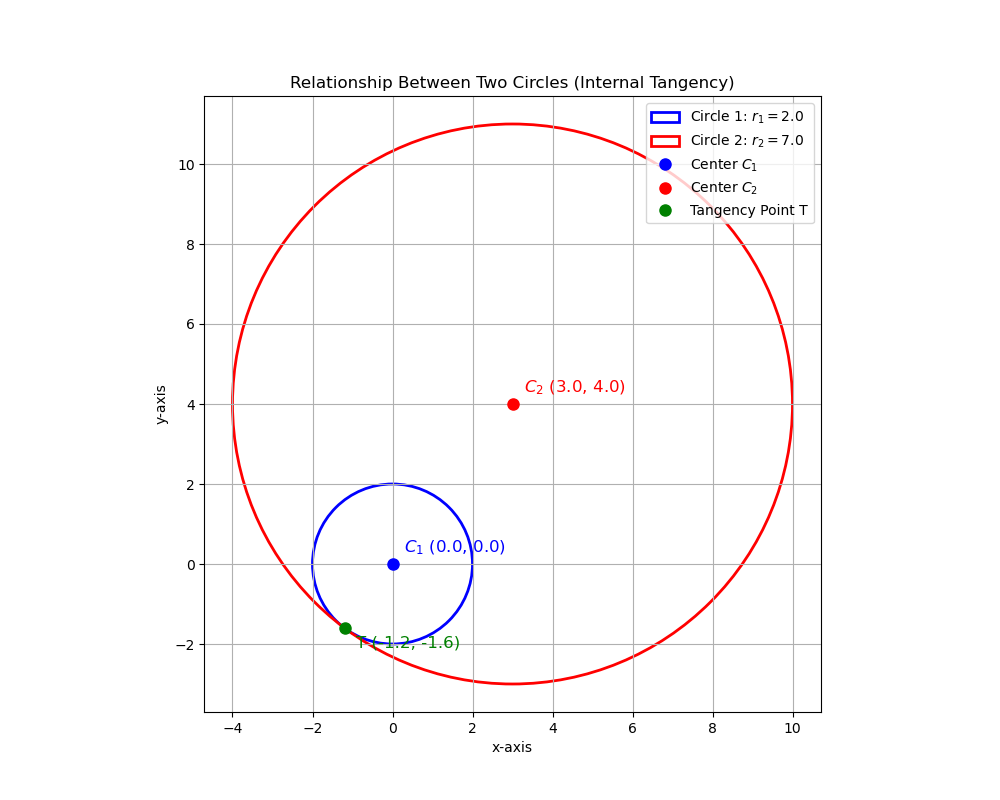
\includegraphics[height=0.5\textheight, keepaspectratio]{figs/figure1.png}
    \label{figure_1}
\end{figure}

\end{document}